
\subsection{Szwarc-Boryczka Algorithm}

\begin{frame}
    \frametitle{Szwarc-Boryczka Algorithm \cite{szwarc_novel_2022}}

    \note<1->[item]{
        Solution Vectors: \begin{itemize}
            \item Paths as list of nodes \begin{itemize}
                      \item Means that they can be different sizes
                  \end{itemize}
        \end{itemize}
    }
    \note<2->[item]{
        Objective function: \begin{itemize}
            \item Path Score
        \end{itemize}
    }

    \begin{itemize}
        \item<1-> Solution Vectors $\Rightarrow$ List of nodes in path
        \item<2-> Objective Function $\Rightarrow$ Path score
    \end{itemize}
\end{frame}

\begin{frame}
    \frametitle{Example}

    \note<1>[item]{
        State of the algorithm after some amount of steps \begin{itemize}
            \item Red and blue Path
        \end{itemize}
    }
    \note<2>[item] {
        Want to create new path \begin{itemize}
            \item Start at origin
            \item Search which nodes follow origin in the paths we have \begin{itemize}
                      \item[$\Rightarrow$] 10 and 5
                  \end{itemize}
            \item Weighted distribution by score of the path the nodes come from
        \end{itemize}
    }
    \note<3>[item]{
        Randomly choose 5 \begin{itemize}
            \item Was the less likely scenario but still could happen
            \item We continue like this
        \end{itemize}
    }
    \note<4>[item]{
        Randomly choose 9 \begin{itemize}
            \item 9 does not appear in the red path
            \item Now we have only node 6 to go to
        \end{itemize}
    }
    \note<5>[item]{
        Choose 6 \begin{itemize}
            \item Now node 3 from path 1 and End from path 2
            \item Don't want to end prematurely so we disregard the end node for now
        \end{itemize}
    }
    \note<6>[item]{
        Choose 3 \begin{itemize}
            \item Only end node from path 1
            \item No other node left to go to
        \end{itemize}
    }

    \note<7>[item]{
        Look at unvisited nodes \begin{itemize}
            \item Want to pick one of them instead if we have enough capacity left
            \item[$\Rightarrow$] Rank them by how promising they are
        \end{itemize}
    }

    \note<8>[item]{
        First Point: Remove nodes that violate capacity \begin{itemize}
            \item In this case, say 1 violates it
        \end{itemize}
    }
    \note<8>[item]{
        Second point: Ranking nodes \begin{itemize}
            \item Need to rely on heuristics
        \end{itemize}
    }
    \note<9-11>[item]{Higher profit}
    \note<10-11>[item]{
        Closer to score center of gravity \begin{itemize}
            \item Algorithm assumes nodes have coordinates
            \item Weighted sum over the nodes' coordinates \begin{itemize}
                      \item Weight = Score
                  \end{itemize}
            \item Marked as a little X
        \end{itemize}
    }
    \note<11>[item]{
        Closer to last visited node \begin{itemize}
            \item Clear winner
        \end{itemize}
    }
    \note<12>[item]{
        Choose 10 \begin{itemize}
            \item Only node 5 saved \begin{itemize}
                      \item Already in use
                      \item[$\Rightarrow$] Again no nodes left
                  \end{itemize}
            \item We could do the whole process again but takes too much time right now
            \item Go to the end
        \end{itemize}
    }
    \note<13>[item]{
        Evaluate score of path \begin{itemize}
            \item Best path so far
            \item Replace worst saved path
        \end{itemize}
    }

    \centering
    \begin{columns}
        \begin{column}{0.48\textwidth}
            \begin{tabular}{r|ccccccc|l}
                \textbf{Path}                          & 1                   & 2                     & 3                     & 4                     & 5                    & 6                    & 7                  & \textbf{Score}                                      \\\hline
                \textcolor{red}{$1$}                   & \textcolor{red}{O}  & \textcolor{red}{$10$} & \textcolor{red}{$5$}  & \textcolor{red}{$4$}  & \textcolor{red}{$6$} & \textcolor{red}{$3$} & \textcolor{red}{E} & 28                                                  \\
                \only<-13>{\textcolor{blue}{$2$}       & \textcolor{blue}{O} & \textcolor{blue}{$5$} & \textcolor{blue}{$9$} & \textcolor{blue}{$6$} & \textcolor{blue}{E}  &                      &                    & 20             \only<2->{\\}}
                \only<2->{\only<2-13>{$*$}\only<14>{2} & \only<2->{O}        & \only<3->{5}          & \only<4->{9}          & \only<5->{6}          & \only<6->{3}         & \only<12->{10}       & \only<13->{E}      & \only<13->{33}}
            \end{tabular}
            \vspace{3mm}

            \visible<8-11>{
                \textbf{Heuristics:}
                Prefer nodes\dots
                \begin{itemize}
                    \item<9-> with higher profit
                    \item<10-> closer to center of gravity
                    \item<11-> closer to current node
                \end{itemize}
            }
        \end{column}
        \begin{column}{0.48\textwidth}
            \begin{tikzpicture}
                \node[draw,shape=circle,minimum size=7mm] (origin) at (0,0) {O};
                % left
                \node[draw,shape=circle,minimum size=7mm] (10) at (-2,0) {10};
                % top left		
                \node[draw,shape=circle,minimum size=7mm] (3) at (-2,2) {3};
                % top		
                \node[draw,shape=circle,minimum size=7mm] (6) at (0,2) {6};
                % right
                \node[draw,shape=circle,minimum size=7mm] (4) at (2,0) {4};
                % bottom
                \node[draw,shape=circle,minimum size=7mm] (5) at (0,-2) {5};
                % bottom right
                \node[draw,shape=circle,minimum size=7mm] (9) at (2,-2) {9};
                % top right
                \node[draw,shape=circle,minimum size=7mm] (1) at (2,2) {1};
                % bottom left
                \node[draw,shape=circle,minimum size=7mm] (end) at (-2,-2) {E};

                \only<1> {
                    \draw[->,red] (origin) -- (10) -- (5) -- (4) -- (6) -- (3) to[bend right] (end);
                    \draw[->,blue] (origin) -- (5) -- (9) -- (6) -- (end);
                }

                \only<2>{
                    \draw[->,red] (origin) -- (10);
                    \draw[->,blue] (origin) -- (5);
                }

                \only<3>{
                    \draw[->] (origin) -- (5);
                    \draw[->,red] (5) -- (4);
                    \draw[->,blue] (5) -- (9);
                }

                \only<4>{
                    \draw[->] (origin) -- (5) -- (9);
                    \draw[->,blue] (9) -- (6);
                }

                \only<5>{
                    \draw[->] (origin) -- (5) -- (9) -- (6);
                    \draw[->,red] (6) -- (3);
                    \draw[->,blue] (6) -- (end);
                }

                \only<6>{
                    \draw[->] (origin) -- (5) -- (9) -- (6) -- (3);
                    \draw[->,red] (3) to[bend right] (end);
                }

                \only<7-11>{
                    \draw[->] (origin) -- (5) -- (9) -- (6) -- (3);
                    \draw[->,dashed] (3) to (10);
                    \draw[->,dashed] (3) to (4);
                }
                \draw<7>[->,dashed] (3) to[bend left] (1);
                \node<10>[minimum size=7mm] (end) at (-0.85,0) {$\times$};

                \only<12>{
                    \draw[->] (origin) -- (5) -- (9) -- (6) -- (3) -- (10);
                    \draw[->,red] (10) -- (5);
                }

                \only<13->{
                    \draw[->] (origin) -- (5) -- (9) -- (6) -- (3) -- (10) -- (end);
                }

                \draw<14>[->,red] (origin) -- (10) -- (5) -- (4) -- (6) to[bend right] (3) -- (3) to[bend right] (end);

            \end{tikzpicture}
        \end{column}
    \end{columns}
\end{frame}

\begin{frame}
    \frametitle{Generalization}

    \note<1->[item]{
        Navigation is the same as the S-Algorithm \begin{itemize}
            \item Requires Triangle-Inequality to decide whether a node can be taken
        \end{itemize}
    }
    \note<2->[item]{
        Center of gravity heuristic requires euclidean graph \begin{itemize}
            \item Weighted sum of \textbf{coordinates}
        \end{itemize}
    }
    \note<2->[item]{
        Other parts to the algorithm that are difficult outside of euclidean
    }
    \note<3->[item] {
        We can try removing thes heuristics \begin{itemize}
            \item Might worsen results
            \item Would need to check experimentally
        \end{itemize}
    }

    \begin{columns}
        \begin{column}{0.48\textwidth}
            \begin{itemize}
                \item<1-> Navigation like S-Algorithm \begin{itemize}
                    \item[$\Rightarrow$] Requires Triangle-Inequality
                \end{itemize}
                \item<2-> Center of gravity heuristic \begin{itemize}
                    \item[$\Rightarrow$] \textcolor{red}{Requires Euclidean Graph}
                \end{itemize}
                \item<3-> Can remove heuristics \begin{itemize}
                    \item Might need to accept worse results
                \end{itemize}
            \end{itemize}
        \end{column}
        \begin{column}{0.48\textwidth}
            \includegraphics<1,3>[width=0.7\textwidth]{res/kaisya_komaru_woman.png}
            \includegraphics<2>[width=0.7\textwidth]{res/kaisya_woman_bad.png}
        \end{column}
    \end{columns}

\end{frame}